\documentclass[11pt]{article}

\usepackage[review]{acl}
\usepackage{times}
\usepackage{latexsym}
\usepackage[T1]{fontenc}
\usepackage[utf8]{inputenc}
\usepackage{microtype}
\usepackage{inconsolata}
\usepackage{graphicx}
\usepackage{booktabs}
\usepackage{array}

\title{Discovering Syntactic Failure Cases in Language Models\\
via Reinforcement Learning}

\author{Yilin An}

\begin{document}
\maketitle
\begin{abstract}
Subject--verb agreement provides a focused setting for finding syntactic
failure cases in language models. This project studies whether reinforcement
learning can guide the discovery of agreement minimal pairs that expose
model weaknesses more effectively than a hand-controlled benchmark. The search
space is symbolic rather than free-form: an RL agent edits syntactic structures,
which are then realized as grammatical/ungrammatical sentence pairs and scored
by a language model. We introduced distribution-aware
generation with subtype quotas and evaluated the resulting 240-example RL
dataset against a 240-example controlled benchmark under matched subtype
coverage. Across \texttt{distilgpt2} and \texttt{gpt2}, RL-discovered examples
are slightly but consistently harder overall than benchmark examples by
accuracy and failure rate. Subtype analysis shows that discovered failures concentrate in
plural-embedded relative clauses and selected PP-attractor structures. The
results suggest that RL can serve as a useful failure-case discovery tool when
paired with coverage controls and sanity checks.
\end{abstract}

\section{Introduction}

Agreement is a simple grammatical dependency on the surface, but it becomes a
useful probe of syntactic competence when distractor nouns or embedded clauses
intervene between the subject and the verb. A language model that only relies
on local heuristics may incorrectly prefer \emph{The dog near the cars run} to
\emph{The dog near the cars runs}. For this reason, subject--verb agreement
has been widely used as a targeted evaluation for whether language models
encode hierarchical syntactic information rather than only surface statistics
\citep{linzen2016assessing,gulordava2018colorless,warstadt2020blimp}.

This project frames agreement evaluation as a failure-case discovery problem.
Rather than only asking how models perform on a fixed benchmark, I ask whether
an RL-guided search procedure can actively discover syntactic minimal pairs
that expose model weaknesses. The intended use of RL is not to train a language
model, but to search over a small symbolic space of syntactic structures. The
system builds grammatical and ungrammatical minimal pairs, scores them with a
target language model, and rewards structures that lead to model failures or
near-boundary decisions.

The central hypothesis is that RL-guided search can discover agreement failure
cases that are harder than a benchmark under matched subtype coverage. The
matched-coverage condition is important: a generated set that is hard only
because it collapses to one subtype is not a fair discovery result. Early
experiments did show this kind of collapse, especially toward object-relative
clauses. I therefore extended the generator to produce a larger
distribution-aware RL dataset with the same size and subtype distribution as
the benchmark. I then ran benchmark-vs-RL evaluation with three Hugging Face
causal language models: \texttt{sshleifer/tiny-gpt2}, \texttt{distilgpt2},
and \texttt{gpt2}.

The main result is that RL-discovered cases are harder overall than benchmark
cases for the two stronger models, \texttt{distilgpt2} and \texttt{gpt2},
although the effect is modest for DistilGPT-2. The weakest model,
TinyGPT-2, fails almost all RL examples, but sanity checks show no duplicate,
lexical-collapse, or grammar-metadata bug; instead, the pattern is best treated
as evidence that the very small model is sensitive to artifacts of the
generated data. Subtype analysis further shows that the discovered failures
are concentrated in plural-embedded relative clauses and PP-attractor cases
such as \texttt{pp\_plural\_attractor\_with},
\texttt{pp\_plural\_attractor\_near},
\texttt{pp\_plural\_attractor\_behind}, and
\texttt{pp\_singular\_attractor\_with}.

\section{Related Work}

Targeted syntactic evaluation has often used minimal pairs: a model succeeds
when it assigns higher probability to a grammatical sentence than to a matched
ungrammatical one. \citet{linzen2016assessing} used number agreement as a
diagnostic for recurrent networks, showing that models can perform well in
simple contexts while still struggling with attractors. \citet{gulordava2018colorless}
extended this style of evaluation with nonce sentences, separating syntactic
generalization from lexical memorization. BLiMP \citep{warstadt2020blimp}
provided a broad benchmark of English minimal pairs, including agreement
phenomena, and helped establish minimal-pair scoring as a common intrinsic
evaluation method.

This project follows the minimal-pair evaluation tradition but focuses on
failure discovery. Instead of only evaluating a fixed benchmark, it asks
whether a search procedure can discover additional challenging cases. The RL component
is deliberately lightweight and interpretable, closer to tabular control over
syntactic templates than to neural text generation \citep{sutton2018reinforcement}.
This is useful for a class
project setting because generated examples remain inspectable: every example
has a template type, subtype, dependency-distance bucket, clause depth, and
controlled grammatical/ungrammatical sentence pair. The work is also related
to adversarial evaluation, but the emphasis here is on fair comparison under
matched syntactic coverage rather than on unrestricted adversarial text.

\section{Method}

\subsection{Data}

The benchmark dataset is a controlled agreement set of 240 BLiMP-style minimal
pairs generated from symbolic templates. It is balanced across three broad
template families: 80 simple-agreement examples, 80 PP-attractor examples, and
80 relative-clause examples. The subtype inventory contains 15 categories:
simple singular and plural agreement; eight PP-attractor subtypes crossing
attractor direction and preposition; and five relative-clause subtypes,
including plural embedded-subject variants.

The final RL dataset also contains 240 examples. It was produced by a
distribution-aware generation mode that uses the benchmark subtype distribution
as a target. The achieved RL distribution exactly matches the target
distribution: 40 examples each for \texttt{simple\_singular} and
\texttt{simple\_plural}; 10 examples for each PP-attractor subtype; and 16
examples for each relative-clause subtype. This gives 80 examples in each
template family and no coverage gaps.

\begin{table}[t]
\centering
\small
\begin{tabular}{lrr}
\toprule
Template family & Benchmark & RL \\
\midrule
Simple agreement & 80 & 80 \\
PP attractor & 80 & 80 \\
Relative clause & 80 & 80 \\
\midrule
Total & 240 & 240 \\
\bottomrule
\end{tabular}
\caption{Benchmark and distribution-aware RL datasets have matched
template-family counts. Subtype counts are also matched exactly.}
\label{tab:data}
\end{table}

\subsection{RL Failure-Case Discovery}

The discovery procedure operates over syntactic structures rather than free-form text.
An environment state records the template type, dependency distance, attractor
count, clause depth, and subtype. Actions select or modify the structure, for
example by choosing a PP template, changing the preposition, selecting a
relative pronoun, or stopping to realize a final minimal pair. When the agent
stops, the system realizes a grammatical sentence and an ungrammatical
counterpart that differ in the intended agreement target.

The initial RL search could find hard cases but produced a narrow
distribution. To address this, I added subtype quotas. The final generation
loop keeps target counts for each subtype and continues until the quotas are
filled or a maximum-attempt budget is reached. Candidate examples are ranked
using model failure, boundary proximity, margin pressure, and simple diversity
terms: underrepresented subtypes receive a bonus, while overrepresented
subtypes are penalized. This modification is heuristic, but it made the output
substantially easier to interpret discovered failures because the final RL
dataset preserves the same subtype support and counts as the benchmark.

\subsection{Models and Scoring}

I evaluate three GPT-2-style causal language models through the same Hugging
Face scoring interface \citep{radford2019language}:
\texttt{sshleifer/tiny-gpt2}, \texttt{distilgpt2}, and
\texttt{gpt2}. For each minimal pair, the scorer computes sentence scores from
next-token log probabilities and counts the pair as correct if the grammatical
sentence receives a higher score than the ungrammatical sentence. Scores are
normalized by token count.

The main metrics are accuracy, failure rate, near-failure rate, and mean
preference margin. Accuracy is the proportion of pairs for which the model
prefers the grammatical sentence. Failure rate is one minus accuracy.
Near-failure rate is the proportion of examples with an absolute preference
margin below a small threshold, indicating boundary cases. Mean preference
margin is the average grammatical-minus-ungrammatical score; higher positive
values indicate stronger preference for the grammatical sentence.

\subsection{Sanity Checks}

Because generated examples can introduce artifacts, I added a sanity-check
pipeline before interpreting the final comparison. It checks dataset size,
subtype and template distributions, duplicate sentences or pairs, repeated
lexical patterns, pair-level grammar validation, and model disagreement
patterns. The final RL dataset shows no subtype collapse, no lexical collapse,
no duplicate or near-duplicate evidence, and no grammar/metadata validation
errors. The main warning is model-specific: TinyGPT-2 has extreme failures on
RL examples, suggesting weak-model artifact exploitation.

\section{Results}

\subsection{Overall Failure Discovery Results}

Table~\ref{tab:overall} shows whether RL search discovers examples that are
harder than the controlled benchmark under matched coverage. RL is marked
harder only when RL accuracy is lower and/or RL failure rate is higher. The RL
dataset is harder for all three models by this definition, but the effect
differs sharply by model.

\begin{table}[t]
\centering
\small
\begin{tabular}{lrrrr}
\toprule
Model & Bench. Acc. & RL Acc. & Bench. Fail & RL Fail \\
\midrule
TinyGPT-2 & 0.471 & 0.017 & 0.529 & 0.983 \\
DistilGPT-2 & 0.762 & 0.758 & 0.237 & 0.242 \\
GPT-2 & 0.846 & 0.792 & 0.154 & 0.208 \\
\bottomrule
\end{tabular}
\caption{Overall benchmark-vs-RL results on 240 examples per dataset.
RL-discovered examples are harder overall for DistilGPT-2 and GPT-2, while TinyGPT-2
shows extreme behavior that is treated as a weak-model artifact caveat.}
\label{tab:overall}
\end{table}

For DistilGPT-2, the difference is small: accuracy drops from 0.762 on the
benchmark to 0.758 on RL, and failure rate rises from 0.237 to 0.242. For
GPT-2, the effect is larger: accuracy drops from 0.846 to 0.792, while failure
rate rises from 0.154 to 0.208. TinyGPT-2 drops from 0.471 benchmark accuracy
to 0.017 on RL. Since the sanity analysis shows that stronger models do not
share this extreme behavior, I do not interpret TinyGPT-2 as the main evidence
for syntactic difficulty.

\begin{figure}[t]
\centering
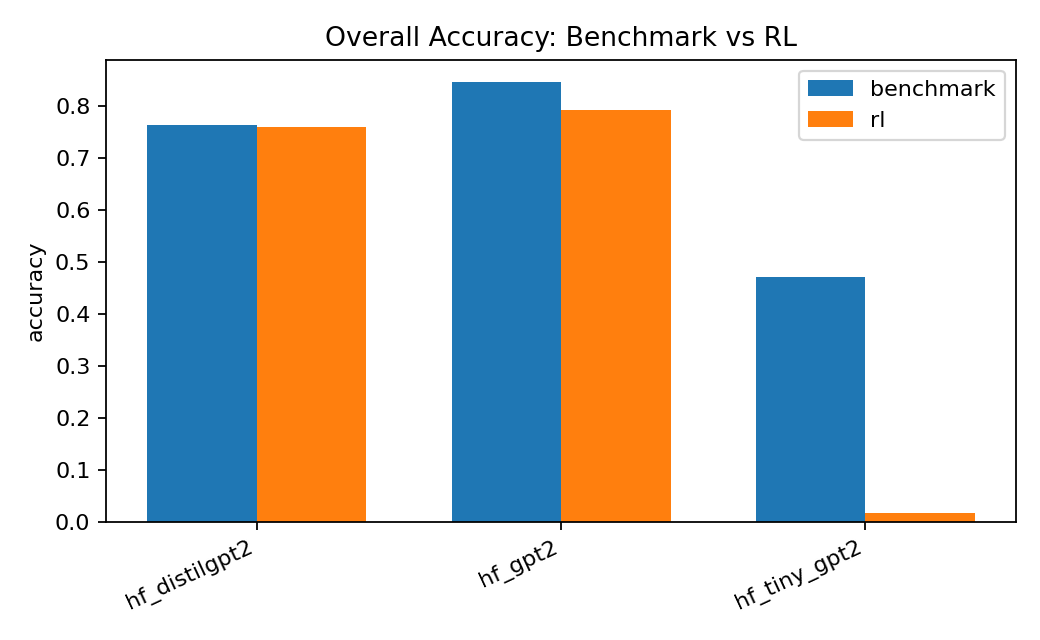
\includegraphics[width=\columnwidth]{outputs/benchmark_vs_rl/figures/benchmark_vs_rl_overall_accuracy_benchmark_vs_rl.png}
\caption{Overall accuracy for benchmark and RL datasets across the GPT-family
models.}
\label{fig:overall}
\end{figure}

\subsection{Subtype-Level Effects}

The harder cases are not evenly distributed across the subtype inventory.
Table~\ref{tab:subtypes} lists selected subtypes where RL-discovered cases were harder for
DistilGPT-2 or GPT-2. The most important shared pattern is that
plural-embedded relative clauses become substantially harder in the RL set,
especially \texttt{object\_relative\_clause\_plural\_embedded\_that}.
For GPT-2, this subtype drops from 0.750 benchmark accuracy to 0.375 on RL.
For DistilGPT-2, it drops from 0.500 to 0.312.

\begin{table*}[t]
\centering
\small
\begin{tabular}{llrrrr}
\toprule
Model & Subtype & Bench. Acc. & RL Acc. & Acc. $\Delta$ & Fail $\Delta$ \\
\midrule
DistilGPT-2 & object\_relative\_clause\_plural\_embedded\_that & 0.500 & 0.312 & -0.188 & 0.188 \\
DistilGPT-2 & pp\_plural\_attractor\_with & 0.700 & 0.300 & -0.400 & 0.400 \\
DistilGPT-2 & pp\_singular\_attractor\_with & 0.900 & 0.800 & -0.100 & 0.100 \\
GPT-2 & object\_relative\_clause\_plural\_embedded\_that & 0.750 & 0.375 & -0.375 & 0.375 \\
GPT-2 & object\_relative\_clause\_plural\_embedded\_who & 0.625 & 0.500 & -0.125 & 0.125 \\
GPT-2 & pp\_plural\_attractor\_with & 0.800 & 0.400 & -0.400 & 0.400 \\
GPT-2 & pp\_plural\_attractor\_near & 0.600 & 0.500 & -0.100 & 0.100 \\
\bottomrule
\end{tabular}
\caption{Selected shared subtypes that are harder in RL than benchmark for
the stronger models. Negative accuracy delta means RL is harder.}
\label{tab:subtypes}
\end{table*}

\subsection{Concrete Failure Cases}

Inspecting individual examples helps explain why the RL search finds these
regions. In the subtype
\texttt{object\_relative\_clause\_plural\_embedded\_that}, the grammatical
main subject is singular, but the embedded subject is plural and linearly
closer to the main verb. GPT-2 fails examples such as:

\begin{quote}
\small
\textbf{Good:} The musician that the artists trust studies.\\
\textbf{Bad:} The musician that the artists trust study.
\end{quote}

For this pair, GPT-2 assigns a negative preference margin ($-0.254$), meaning
that it prefers the ungrammatical plural verb \emph{study}. This is the kind
of case the RL search is intended to discover: the sentence is still
controlled and grammatical, but it places a misleading plural noun inside an
embedded clause immediately before the agreement decision. Similar failed RL
examples include \emph{The scientist that the neighbors call speaks/speak} and
\emph{The dancer that the mechanics call listens/listen}. These examples are
not lexical duplicates; they instantiate the same structural pressure with
different nouns and verbs.

The PP-attractor subtype \texttt{pp\_plural\_attractor\_with} shows a different
surface configuration. Here the attractor is inside a prepositional phrase
rather than a relative clause:

\begin{quote}
\small
\textbf{Good:} The driver with the letters opens.\\
\textbf{Bad:} The driver with the letters open.
\end{quote}

Both GPT-2 and DistilGPT-2 fail this example, with margins of $-0.456$ and
$-0.345$, respectively. The model appears to be pulled toward the plural
attractor \emph{letters}, even though the true subject head is singular
\emph{driver}. Other examples in the same discovered subtype include
\emph{The actor with the computers opens/open} and \emph{The student with the
cabinets travels/travel}. The repeated structural pattern, rather than a
single lexical item, is what matters.

These examples also clarify why matched subtype coverage is necessary. If the
RL system only produced relative clauses, it would be unclear whether the
generator was discovering generally harder syntactic cases or simply changing
the dataset composition. By forcing the RL dataset to contain the same subtype
counts as the benchmark, failures like the two examples above can be compared
within the same structural categories.

PP-attractor discovery effects are more mixed but still important. The subtype
\texttt{pp\_plural\_attractor\_with} is a clear hard case for both stronger
models: DistilGPT-2 drops from 0.700 to 0.300, and GPT-2 drops from 0.800 to
0.400. Other PP-attractor effects are model- or direction-specific. For
example, \texttt{pp\_plural\_attractor\_near} is harder for GPT-2 in RL, but
easier for DistilGPT-2. In the independent sanity analysis, stronger-model hard
subtypes include \texttt{pp\_plural\_attractor\_with},
\texttt{pp\_plural\_attractor\_near},
\texttt{pp\_plural\_attractor\_behind}, and
\texttt{pp\_singular\_attractor\_with}. This suggests that PP structures form
a broad region of difficulty, but not a uniform one.

The multi-model subtype analysis on the controlled benchmark also supports
this interpretation. On the benchmark alone, the consistently hard subtype
across the three GPT-family models is
\texttt{pp\_plural\_attractor\_behind}. The hardest benchmark subtypes for
DistilGPT-2 include \texttt{pp\_plural\_attractor\_near},
\texttt{pp\_plural\_attractor\_behind}, and
\texttt{object\_relative\_clause\_plural\_embedded\_who}. For GPT-2, the
hardest include \texttt{pp\_plural\_attractor\_behind},
\texttt{pp\_plural\_attractor\_near}, and
\texttt{object\_relative\_clause\_plural\_embedded\_who}. Thus, RL does not
discover difficulty from nowhere; it tends to intensify regions that are already
challenging in the controlled benchmark.

\subsection{Subtype Distribution Across Models}

The distribution of hard subtypes differs across models. On the controlled
benchmark alone, DistilGPT-2's hardest subtypes are
\texttt{pp\_plural\_attractor\_near} and
\texttt{pp\_plural\_attractor\_behind}, both at 0.300 accuracy, followed by
\texttt{object\_relative\_clause\_plural\_embedded\_who} at 0.438. GPT-2 is
stronger overall, but its hardest benchmark subtypes still come from the same
two families: \texttt{pp\_plural\_attractor\_behind} at 0.500,
\texttt{pp\_plural\_attractor\_near} at 0.600, and
\texttt{object\_relative\_clause\_plural\_embedded\_who} at 0.625. Thus, the
RL search is not only exploiting idiosyncratic weaknesses of one model; it
often lands in structural regions that are already difficult for multiple
models.

However, the models do not rank every subtype the same way. For example,
\texttt{pp\_plural\_attractor\_near} becomes harder for GPT-2 in the RL set
(0.600 benchmark accuracy to 0.500 RL accuracy), but easier for DistilGPT-2
(0.300 to 0.600). In contrast, \texttt{pp\_plural\_attractor\_with} is harder
in RL for both stronger models, with the same 0.400 accuracy drop. This
suggests that some discovered failures are model-specific, while others are
more robust across related causal language models. The robust cases are the
most useful ones for a failure-discovery benchmark, because they point to
structural configurations that remain challenging even as model capacity
increases.

\section{Discussion and Conclusion}

The results support the main hypothesis with qualifications. Under matched
subtype coverage, the RL discovery procedure finds examples that are harder
overall than the benchmark for DistilGPT-2 and GPT-2. The effect is not huge
for DistilGPT-2, but it is directionally consistent across accuracy and
failure rate. GPT-2 shows a clearer drop. This suggests that structure-level
RL search can identify agreement examples that expose model weaknesses beyond
a balanced controlled benchmark.

At the same time, the project also shows why automatic failure discovery needs
careful controls. The first RL outputs were not suitable for a fair comparison
because they concentrated too heavily in one subtype. The final
distribution-aware generator fixed this by matching benchmark subtype counts.
Sanity checks were also necessary: without them, TinyGPT-2's near-total RL
failure could be mistaken for the central result. The better interpretation is
that TinyGPT-2 is too weak and artifact-sensitive to serve as the main evidence
for syntactic difficulty. The stronger models give a more stable picture.

Subtype analysis is the most informative part of the failure discovery story. Simple
agreement is generally easy, while PP-attractor and relative-clause structures
carry most of the difficulty. The strongest RL effects appear in
plural-embedded relative clauses and in selected PP-attractor subtypes,
especially \texttt{pp\_plural\_attractor\_with}. These results are compatible
with the idea that harder agreement cases combine long-distance dependencies
with misleading local number cues.

This study is limited by scale. The dataset is controlled and interpretable,
but still small relative to standard benchmarks. The RL policy is also a
lightweight search mechanism over hand-designed templates, not an open-ended
generator. Future work could add more syntactic phenomena, compare against
larger instruction-tuned models on hardware that can support them, and use
human validation for generated examples. Even within these limits, the project
shows that RL-guided failure discovery can be useful when paired with distribution
matching and error analysis.

\section*{Statement of Contributions}

I implemented the controlled agreement generation pipeline, the structure-level
RL environment and Q-learning search, the distribution-aware RL generation
mode, the benchmark-vs-RL comparison pipeline, multi-model Hugging Face
evaluation, subtype-level summaries, plotting, and sanity-check/error-analysis
scripts. I also ran the reported experiments, inspected the generated outputs,
and wrote this report. The project uses standard open-source models and
libraries; no external API-based model results are included in the main
reported numbers.

\bibliography{custom}

\end{document}
